\documentclass[11pt]{article}

\usepackage[margin=1in]{geometry}
\usepackage[T1]{fontenc}
\usepackage[utf8]{inputenc}
\usepackage{lmodern}
\usepackage{amsmath}
\usepackage{amssymb}
\usepackage{graphicx}
\usepackage{booktabs}
\usepackage{natbib}
\usepackage[hidelinks]{hyperref}
\usepackage{xurl}

\title{Curvature-tuned persistent homology and embedding of percolation complexes on $\{3,q\}$ tilings}
\author{Zachary Treisman}
\date{\today}

\begin{document}

\maketitle

\begin{abstract}
A percolation cluster on an exponentially growing graph is a random subgraph whose loop content can be substantial. Representing it faithfully, whether combinatorially as a filtered simplicial complex or concretely as coordinates in a vector space, costs something whenever the cluster is not a tree. This paper measures that cost as a function of curvature, using the regular $\{3,q\}$ triangle tilings as a one-parameter family running from flat and amenable ($q=6$) to deeply hyperbolic ($q=20$). A single growth-rate parameter $\lambda(q)$ governs every result below. Total persistent $H_1$ of the bond-percolation complex on these tilings collapses onto a closed-form law in $1/\lambda(q)$. An identity that reduces total loop persistence to the weight of the lattice's minimum spanning tree, minus a provably exact boundary correction, turns most of that law from a fit into a derivation, and finite-size convergence itself splits cleanly along the amenable/nonamenable line. The same suppression then shows up in an actual embedding: percolation clusters mapped into a vector space by a branching random walk produce loop-holonomy that falls with curvature in step with $H_1$, and that suppression propagates into the feature-splitting behavior of a sparse autoencoder trained on the embedded clusters. 
\end{abstract}

\section{Introduction}
\label{sec:intro}

A tree embeds into a vector space with zero distortion: a branching random walk, or any construction that assigns each node the cumulative sum of independent steps along its unique path from a root, reproduces the tree's own path metric exactly. This is one reason hierarchical data is so often modeled as, or embedded via, tree structure: Poincar\'{e} embeddings place hierarchies in hyperbolic space specifically to preserve tree distances \citep{nickel2017}, and synthetic data models are sometimes built directly from percolation clusters on the assumption that those clusters are themselves close to tree-shaped. But most naturally occurring branching structures are not exactly trees. A percolation cluster is a random subgraph of some ambient graph, and whether it looks tree-like depends on how likely random paths within it are to reconnect and close a loop. When they do, an embedding built on the tree assumption pays for it: coordinates that would agree if the cluster really were a tree instead disagree by however much the loop's holonomy fails to close.

This cost is intuitive but rarely turned into a measurable quantity for a specific graph family. This paper does that, using the regular hyperbolic tilings $\{3,q\}$ (equilateral-triangle tessellations with $q$ triangles meeting at every vertex) as a curvature dial. Varying $q$ from $6$ (flat, amenable) through increasingly negatively curved values interpolates continuously between loop-rich and asymptotically tree-like percolation behavior, through a single, computable growth-rate parameter $\lambda(q)$ (\S\ref{sec:curvature-knob}). $\lambda(q)=1$ at $q=6$ and $\lambda(q)>1$ for every $q\ge7$, so this dial sits directly on top of the amenable/nonamenable distinction that governs whether percolation on the tiling exhibits mean-field critical behavior \citep{hutchcroft2019}: it is tied to a known, provable threshold, not chosen arbitrarily.

Two results follow, measured two different ways.

\textbf{Result A} (\S\ref{sec:partA}) treats loop content as a property of the abstract combinatorial object. Bond percolation is built as a single filtered simplicial complex, and its total persistent $H_1$ (summed bar length across the whole percolation process, per vertex) is measured across twelve values of $q$ and a range of system sizes per $q$. The result is a closed-form law in $1/\lambda(q)$, and an identity turns most of that law into a derivation rather than a fit: total $H_1$ persistence reduces algebraically to the weight of the lattice's minimum spanning tree minus a boundary correction, and the boundary correction alone can be shown to carry a $1/\lambda(q)$ dependence with a derived coefficient. Finite-size convergence turns out to split cleanly at the amenable/nonamenable line as well, a second, unanticipated confirmation of the same boundary.

\textbf{Result B} (\S\ref{sec:partB}) asks what happens once a percolation cluster is no longer just an abstract complex but an actual point cloud. Each cluster is embedded into a vector space via a branching random walk along its spanning tree, and the resulting embedding's loop-holonomy is measured directly, with no homology computation involved. That holonomy falls with curvature in the same order as $H_1$ does. More consequentially, the same suppression is visible three steps downstream, in the feature-splitting behavior of a sparse autoencoder trained on the embedded clusters.

That both results move together should not be assumed automatically. $H_1$ in Result A is a property of the abstract percolation complex, independent of any embedding, while Result B is a property of one specific embedding (branching random walk) and one specific trained model, and embeddings can create or destroy loop structure relative to the underlying complex. Agreement between the two is therefore a real, if modest, finding rather than a tautology.

Section~\ref{sec:diagnostic} sets up persistent homology as the diagnostic used throughout. Section~\ref{sec:curvature-knob} defines the curvature dial and its growth rate $\lambda(q)$. Sections~\ref{sec:partA} and \ref{sec:partB} present Results A and B. Section~\ref{sec:brill} discusses one concrete application of these results: percolation-based synthetic data models for mechanistic interpretability research, which rely on the same tree-likeness assumption measured here, currently justified only asymptotically in ambient dimension.

\section{Persistent homology as the diagnostic}
\label{sec:diagnostic}

Bond percolation defines a natural filtration. Given a graph $G$, assign each edge $e\in G$ an i.i.d.\ Uniform$[0,1]$ occupation threshold $u_e\in[0,1]$, and build the clique (flag) complex of the graph using those thresholds as filtration values. Declare edge $e$ occupied at parameter $p$ whenever its threshold $u_e\le p$, and declare 2-simplices occupied wherever a triangle's three edges are all present. A triangle enters the filtration at the maximum of its three edge thresholds. Reusing the same draw of thresholds across all $p$ makes the occupied sets nested: one draw of $\{u_e\}$ gives a single filtration that encodes the entire coupled percolation process across every value of $p$. Standard persistent homology software (here, GUDHI) extracts persistent $H_0$ and $H_1$ from that one filtration directly, as Betti curves $\beta_0(p)$, $\beta_1(p)$ and persistence diagrams whose bars record when each loop is born and when it gets filled in. Any single draw of $\{u_e\}$ is still one sample path, and the resulting curves fluctuate from draw to draw. The results below average over 12 independent draws per lattice, with the reported spread reflecting that realization-to-realization variation. This connects to existing work on homological percolation, which studies the birth and death of giant cycles in percolation processes via the Euler characteristic curve on cubical and other lattices \citep{bobrowski2020}; the approach here specializes to the $\{3,q\}$ triangulated case and adds curvature as an explicit parameter.

One technical condition makes this tractable: as long as the graph's only 3-cliques are genuine faces of the underlying triangulation (no ``accidental'' triangles among mutually adjacent vertices that don't bound a real 2-cell), the clique complex reconstructs the correct 2-cell structure automatically. This was verified computationally for every lattice used below (Euler characteristic exactly 1 in each case, confirming a topological disk, and an exact match between the graph's 3-cliques and the known face list, with zero spurious or missing triangles).

One subtlety matters again in \S\ref{sec:partA-derivation}. A single triangular face's own 3-cycle is born, in this filtration, only once all three of its edges are present, which is also the threshold at which the 2-simplex fills it in. Isolated triangle loops are therefore born and die simultaneously and contribute zero persistence; whatever loop content survives has to come from cycles spanning more than one face.

\section{Percolation on $\{3,q\}$ tilings}
\label{sec:curvature-knob}

The family of regular triangulations $\{3,q\}$ ($q$ equilateral triangles meeting at every vertex) is built by the standard ring-growth construction: starting from a single vertex, each successive ring is attached according to the fixed combinatorial rule that $q$ triangles meet at every vertex. Ring sizes satisfy the linear recursion
\[
rc[n] = (q-4)\cdot rc[n-1] - rc[n-2], \qquad rc[0]=1,\ rc[1]=q,
\]
whose dominant root
\[
\lambda(q) = \frac{(q-4) + \sqrt{(q-4)^2-4}}{2}
\]
is the tiling's asymptotic per-ring growth rate, $rc[n]/rc[n-1]\to\lambda(q)$ as $n\to\infty$. At $q=6$ the discriminant vanishes, giving a repeated root $\lambda=1$ and linear, rather than exponential, ring growth: the flat, parabolic case. For $q\ge7$ the discriminant is positive and $\lambda>1$, giving exponential growth. Table~\ref{tab:ladder} gives illustrative values.

\begin{table}[htbp]
\centering
\begin{tabular}{lllr}
\toprule
$q$ & geometry & amenable? & $\lambda(q)$ \\
\midrule
6  & flat (Euclidean triangular lattice) & yes & 1.000 \\
7  & mildly hyperbolic & no & 2.618 \\
8  & more hyperbolic & no & 3.732 \\
12 & strongly hyperbolic & no & 8.873 \\
20 & deep hyperbolic & no & 17.944 \\
\bottomrule
\end{tabular}
\caption{The curvature ladder: illustrative values of $q$, from flat to deeply hyperbolic.}
\label{tab:ladder}
\end{table}

For this specific family, regular $\{3,q\}$ tilings, which are Gromov-hyperbolic and quasi-transitive for $q\ge7$, the growth dichotomy is equivalent to amenability, not just correlated with it: a hyperbolic, quasi-transitive graph is amenable if and only if it is elementary (virtually cyclic), and elementary graphs are the ones with at most linear growth, so $\lambda(q)=1$ versus $\lambda(q)>1$ is the amenable/nonamenable distinction for this family. That equivalence is special to this family, though, not a general fact about growth rate and amenability; some amenable groups, such as the lamplighter group, also grow exponentially.

This dichotomy matters for percolation specifically because, on any nonamenable, Gromov-hyperbolic, quasi-transitive graph, there is a phase with infinitely many infinite clusters between two distinct critical probabilities $p_c<p_u$, and the critical exponents at $p_c$ provably take their mean-field, i.e.\ Bethe-lattice, values (Benjamini \& Schramm's conjecture, proved by Tom Hutchcroft \citep{hutchcroft2019}; see also H\"aggstr\"om's survey of Schramm's percolation work \citep{haggstrom}). On the $\{7,3\}$ hyperbolic lattice, concretely, the percolation cluster-size scaling exponent $\tau$ has already been measured to converge to its mean-field value of $5/2$ \citep{mertens2017}. Hyperbolic lattices are mean-field not because of dimension but because non-amenability forces the same ``loops are rare'' structure that high dimension forces in Euclidean space.

The $\{3,q\}$ family therefore gives a single, precisely defined, geometrically interpretable parameter that interpolates between loop-rich (Euclidean, $q=6$) and asymptotically tree-like (deep hyperbolic, $q\to\infty$) percolation regimes: one integer, measurable on graphs small enough to simulate directly.

\section{Result A: the topological loop content of percolated subsets}
\label{sec:partA}

\subsection{Method and validation}

The $\{3,q\}$ graphs used here were built via the ring-growth construction of \S\ref{sec:curvature-knob}. Running it to ring 5 for $q=7$ gives a graph with 617 vertices and 847 faces, an Euler characteristic of exactly 1, confirming the graph is a topological disk, and an exact match between the graph's triangle cliques and its true face list, confirming no spurious triangles. The flat $q=6$ control is a finite patch of the ordinary triangular lattice; the $q=8$ case uses the same construction at one ring fewer (609 vertices), chosen so all three lattices are closely matched in size.

For each lattice, 12 independent percolation realizations (random edge filtrations) were run through the filtered-complex pipeline, and the resulting Betti curves and total persistent-$H_1$ (``loopiness'') statistics were averaged. As a sanity check, the flat lattice's $\beta_0(p)$ crossover lands almost exactly on the lattice's known exact bond-percolation threshold ($p_c\approx0.347$ for the triangular lattice), confirming the pipeline reproduces standard percolation behavior before any curvature is introduced.

\subsection{The scaling law}
\label{sec:scaling-law}

Figure~\ref{fig:euclidean} (\texttt{euclidean\_control\_betti\_curves.png}) shows $\beta_0/N$ and $\beta_1/N$ for the flat control, with the loop-density curve peaking near $p\approx0.7$ and the fragmentation transition crossing the known exact threshold.

\begin{figure}[htbp]
\centering
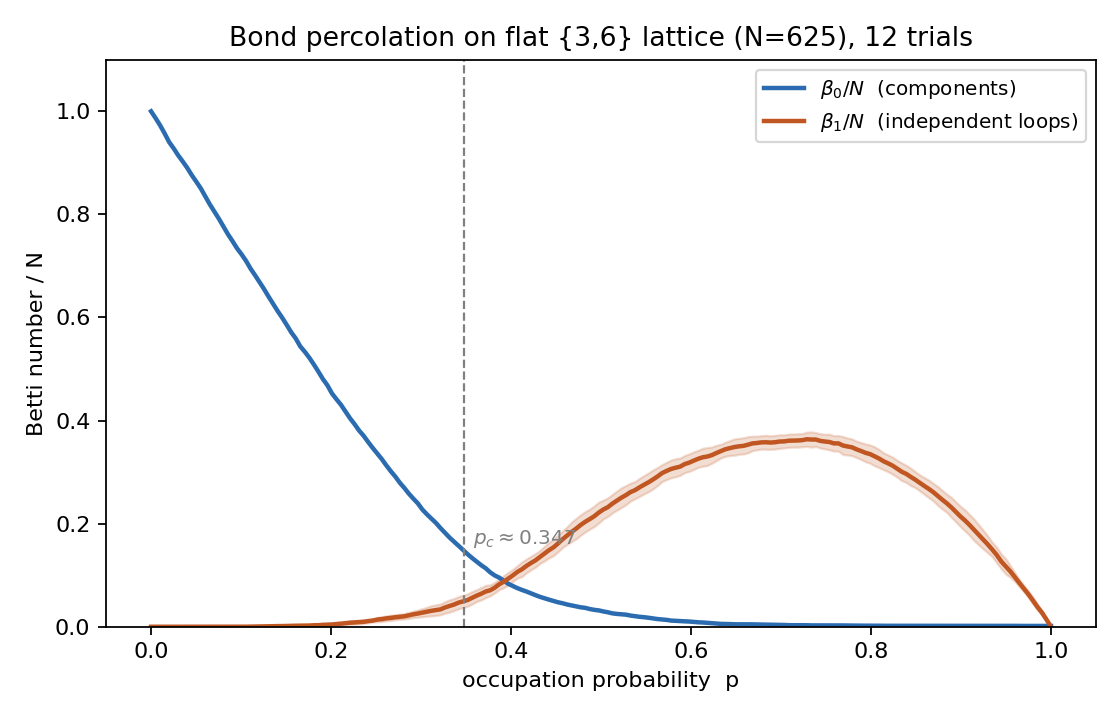
\includegraphics[width=\textwidth]{euclidean_control_betti_curves.png}
\caption{Betti curves $\beta_0/N$ and $\beta_1/N$ for the flat ($q=6$) control lattice.}
\label{fig:euclidean}
\end{figure}

Figure~\ref{fig:comparison} (\texttt{curvature\_persistence\_comparison.png}) is a pilot demonstration at matched system size: the same $\beta_1/N$ curves for $q=6,7,8$ overlaid, and total $H_1$ persistence per vertex plotted against $q$:

\begin{itemize}
\item $q=6$ (flat): $0.160\pm0.007$ total $H_1$ persistence per vertex
\item $q=7$ ($\{3,7\}$): $0.089\pm0.005$
\item $q=8$: $0.076\pm0.002$
\end{itemize}

Loop persistence per vertex falls by roughly 45\% moving from flat to $\{3,7\}$, and continues to fall monotonically and well outside error bars as curvature increases further.

\begin{figure}[htbp]
\centering
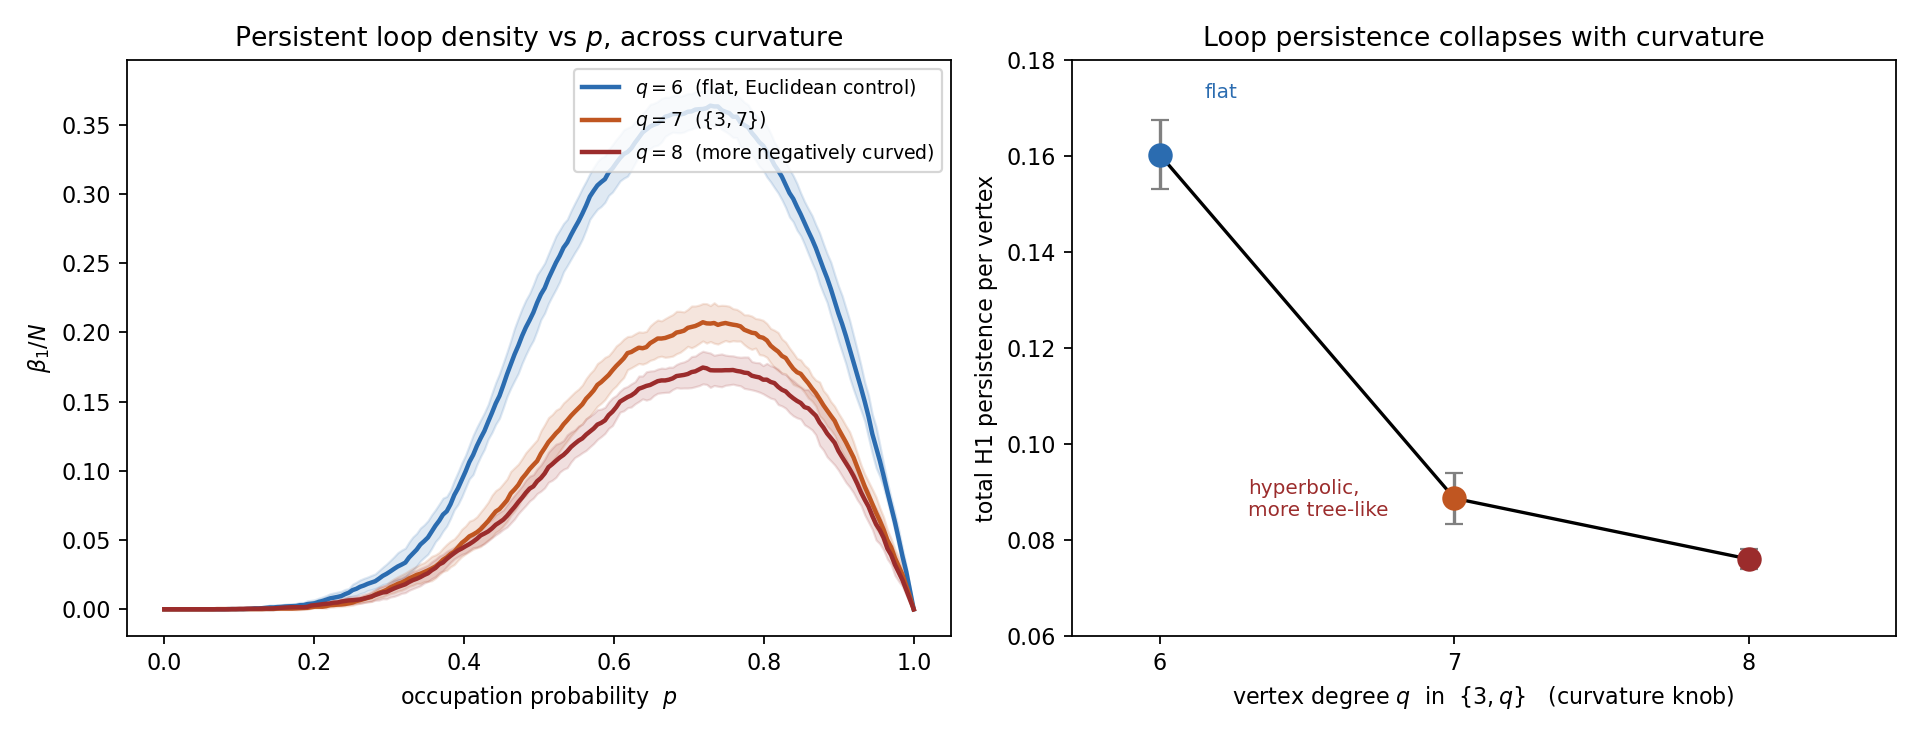
\includegraphics[width=\textwidth]{curvature_persistence_comparison.png}
\caption{$\beta_1/N$ curves for $q=6,7,8$ overlaid, and total $H_1$ persistence per vertex versus $q$.}
\label{fig:comparison}
\end{figure}

A full sweep extends this three-point demonstration to twelve values of $q$ (6 through 20) and, for each $q$, several ring depths spanning roughly two orders of magnitude in system size, from a few hundred vertices up to tens of thousands, to get an explicit scaling law rather than a single matched-size snapshot. Figure~\ref{fig:scaling} (\texttt{curvature\_scaling\_law.png}) shows the result. Using each $q$'s largest available system size (for $q=6$, its converged large-$N$ asymptote from \S\ref{sec:convergence}, since raw sweep sizes for $q=6$ do not converge at any practical ring depth), total $H_1$ persistence per vertex follows
\[
0.0381 + \frac{0.1477}{\lambda(q)}, \qquad R^2=0.9982,
\]
with $\lambda(q)$ as defined in \S\ref{sec:curvature-knob}. The fit has a natural reading: the intercept is a curvature-independent floor, and the $1/\lambda$ term captures everything curvature suppresses, decaying at the tiling's own growth rate. \S\ref{sec:partA-derivation} turns this reading into a derivation, and \S\ref{sec:brill} returns to what the intercept can and cannot be interpreted as.

\begin{figure}[htbp]
\centering
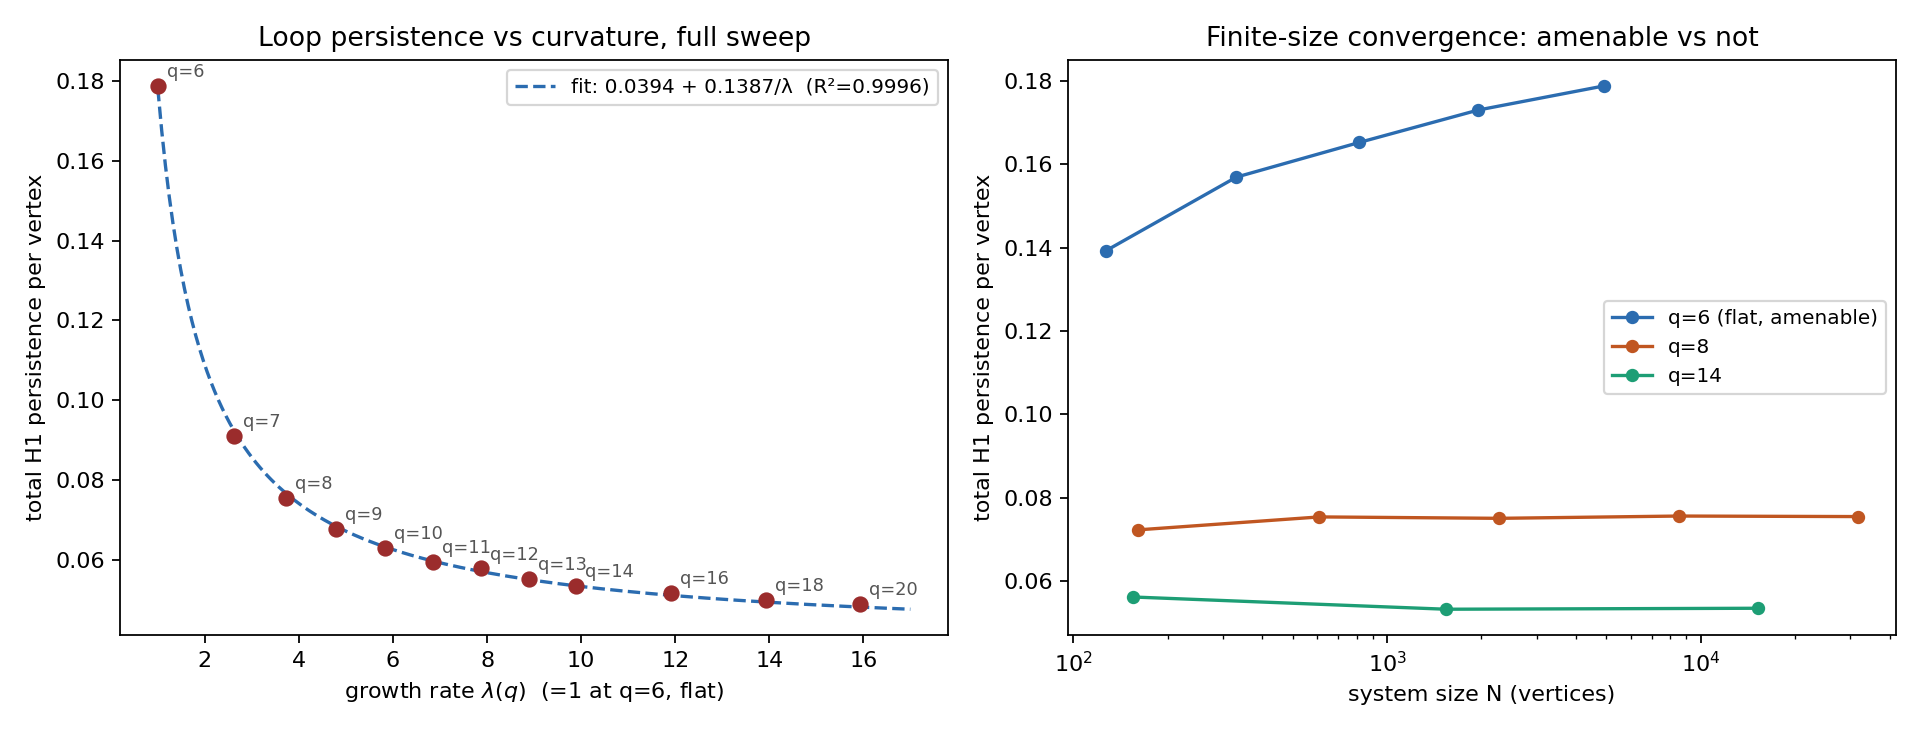
\includegraphics[width=\textwidth]{curvature_scaling_law.png}
\caption{Total $H_1$ persistence per vertex versus $q$: the all-twelve fit (dotted) versus the hyperbolic-only fit excluding $q=6$ (dashed); $q=6$ sits visibly above the hyperbolic trend's extrapolation (left, \S\ref{sec:q6-outlier}). Finite-size convergence for $q=6,8,14$ (right).}
\label{fig:scaling}
\end{figure}

\subsubsection{Is $\lambda(q)$ really the right variable?}
\label{sec:results-check}

A fit this good, with two free parameters over twelve points, invites a simple objection: perhaps any sufficiently flexible decreasing function of $q$ would fit about as well, and $\lambda(q)$'s appearance is an artifact of the fitting range rather than a meaningful choice of variable. This is checkable directly: refit the same two-parameter form, intercept $+$ slope$\,\times f(q)$, against several structurally motivated alternatives to $f(q)=1/\lambda(q)$, and compare $R^2$.

\begin{table}[htbp]
\centering
\begin{tabular}{lr}
\toprule
$f(q)$ & $R^2$ \\
\midrule
$1/\lambda(q)$ \emph{(used above)} & 0.9982 \\
$1/\lambda(q)^2$                    & 0.9670 \\
$1/(q-4)$                           & 0.8849 \\
$1/(q\cdot(q+1))$ (naive one-loop-per-vertex guess) & 0.7950 \\
$1/q^2$                             & 0.8098 \\
$1/q$                               & 0.6962 \\
$e^{-q/5}$                          & 0.6914 \\
\bottomrule
\end{tabular}
\caption{$R^2$ for the same two-parameter fit against alternative variables. $1/\lambda(q)$ is not just the best of these; it clears its closest structural cousin, $1/(q-4)$ (which $\lambda(q)$ asymptotically approaches as $q\to\infty$), by a wide margin.}
\label{tab:altfit}
\end{table}

Table~\ref{tab:altfit} rules out the objection: if the truth here were simply some smooth decreasing function of $q$, several of these alternatives should score comparably. None do. $\lambda(q)$ is also not an arbitrary choice of variable. It is the tiling's exponential growth rate, the same spectral-radius-type quantity that governs generating-function asymptotics (return probabilities, Green's functions) on these graphs, and the quantity Hutchcroft's mean-field theorem hinges on via non-amenability; \S\ref{sec:partA-derivation} makes this connection precise instead of structural.

\subsection{Finite-size convergence splits at the amenability boundary}
\label{sec:convergence}

A second finding was not anticipated going in: finite-size convergence itself splits cleanly along the amenable/nonamenable line. Every nonamenable $q$ tested (7 and up) converges to within 1--2\% almost immediately and stays flat out to systems of tens of thousands of vertices, while $q=6$ drifts upward by more than 3\% between the two largest sizes tested in the original sweep ($N=1951$ to $N=4921$). This is an empirical fingerprint of the isoperimetric distinction at the heart of the Benjamini--Schramm/Hutchcroft result: nonamenable graphs have boundary scaling with volume, so finite-size corrections decay fast; amenable graphs don't have that control, so they don't.

Because the $\{3,q\}$ tilings are deterministic given $q$ and ring depth, the only randomness in this pipeline is the percolation thresholds, averaged over properly at every point. For $q=6$ specifically, this was pushed far beyond the original sweep: seven additional ring depths, up to ring $1000$ ($N\approx3.00\times10^6$), with 8--15 percolation draws per size, parallelized across independent realizations. The combined series, $N=127$ to $N=3{,}003{,}001$, fits cleanly to a power-law approach to a finite asymptote,
\[
H_1/\text{vertex}(N) = A - B/N^\alpha, \qquad A=0.18757\pm0.00034,\ B=0.4164\pm0.0266,\ \alpha=0.4453\pm0.0129 \quad (R^2=0.9988).
\]
So $q=6$ does converge; it simply needs roughly $1000\times$ the vertex count that any hyperbolic $q$ needs, consistent with amenable finite-size corrections decaying as a power of $N$ rather than exponentially fast. The fitted exponent $\alpha\approx0.445$ is close to, though not an exact match for, the $1/\sqrt N$ perimeter-to-area ratio expected of a 2-dimensional disk of $N$ vertices ($\sim4\sigma$ from $1/2$). $A$ is the value used for $q=6$ throughout this paper.

\subsection{$q=6$'s position relative to the hyperbolic trend}
\label{sec:q6-outlier}

$q=6$ is the family's only amenable ($\lambda=1$) point, and it sits at extreme leverage in this fit: $1/\lambda=1$ for $q=6$, versus $1/\lambda\in[0.05,0.38]$ for every hyperbolic $q$ tested. The twelve-point $R^2$ alone should not be trusted without checking this directly. Refitting using only the eleven hyperbolic points ($q\ge7$) gives an \emph{even tighter} law,
\[
H_1/\text{vertex} = 0.0404 + \frac{0.1316}{\lambda(q)}, \qquad R^2=0.9995 \quad (\text{vs.\ }0.9982\text{ for all twelve}),
\]
and extrapolating this hyperbolic-only trend to $\lambda=1$ predicts $H_1/\text{vertex}(6)=0.1721$, which is $0.0155$ below the actual converged value, $0.18757\pm0.00034$ (\S\ref{sec:convergence}): a gap roughly $45$ times the asymptote's uncertainty, too large to be measurement noise (Figure~\ref{fig:scaling}).

This gap is informative rather than a defect in the fit. $q=6$ is the family's unique amenable/parabolic case, and \S\ref{sec:convergence} already showed it behaves qualitatively differently from every hyperbolic $q$ at finite size. \S\ref{sec:partA-derivation}'s decomposition explains why, and checks it independently: the boundary term contributes $-\tfrac14+\tfrac{1}{4\lambda(q)}$, which vanishes identically at $\lambda=1$. In the $N\to\infty$ limit, then, $H_1$/vertex at $q=6$ equals $\mu(6)$ with \emph{zero} boundary correction, so any $q=6$ deviation from the hyperbolic trend has to live entirely in the bulk term. \S\ref{sec:partA-derivation} confirms that this is exactly what happens.

\subsection{Deriving the law: an exact identity}
\label{sec:partA-derivation}

A fit this clean (\S\ref{sec:scaling-law}, $R^2=0.9982$) demands an explanation rather than an appeal to curve-fitting. This section derives one, as far as it goes: the $1/\lambda(q)$ dependence splits into a boundary contribution that is now a proven consequence of the ring-count recursion, and a bulk contribution that is not.

\subsubsection{An exact identity}

Because the percolation complex is a triangulated topological disk (\S\ref{sec:diagnostic}), $\beta_2(p)=0$ identically: a 2-dimensional complex only carries an $H_2$ class around a genuine enclosed void, which requires a closed surface, and a disk's boundary is never closed. Consequently the Euler characteristic $\chi(p)=N-E(p)+F(p)$ (vertices are present at every $p$; $E(p),F(p)$ count edges and triangles occupied by threshold $p$) satisfies $\chi(p)=\beta_0(p)-\beta_1(p)$ exactly, at every $p$, giving
\[
\beta_1(p) = \beta_0(p) - N + E(p) - F(p).
\]
Total $H_1$ persistence is $\int_0^1\beta_1(p)\,dp$, literally the area under the loop-density curve of Figure~\ref{fig:euclidean}. Integrating term by term: writing $u_e$ for edge $e$'s occupation threshold, $E(p)=\sum_e\mathbb{1}[u_e\le p]$ gives $\int_0^1E(p)\,dp=\sum_e(1-u_e)$; writing $m_t=\max(\text{the three edge thresholds of triangle }t)$ for its occupation threshold, $\int_0^1F(p)\,dp=\sum_t(1-m_t)$.

The $\beta_0(p)$ term is the classical single-linkage/Kruskal fact: the connected-component structure of the graph restricted to edges with $u_e\le p$ is, for every $p$, identical to the component structure using only the edges of the graph's minimum spanning tree (MST, the subset of $N-1$ edges connecting all vertices at minimum total weight, built greedily by Kruskal's algorithm in increasing weight order) with weight $\le p$. So $N-\beta_0(p)$ equals the number of MST edges with weight $\le p$, and $\int_0^1\beta_0(p)\,dp = 1+w_{\mathrm{MST}}$, where $w_{\mathrm{MST}}=\sum_{e\in\mathrm{MST}}u_e$.

Assembling the pieces gives an exact identity, not an approximation and not only in expectation, for a single percolation realization:
\begin{equation}
\int_0^1\beta_1(p)\,dp = w_{\mathrm{MST}} - \sum_e u_e + \sum_t m_t.
\label{eq:exact-identity}
\end{equation}
This was checked directly against the GUDHI pipeline: for a $\{3,7\}$ lattice at ring depth 5 ($N=617$), the right-hand side of \eqref{eq:exact-identity} matches GUDHI's computed total $H_1$ persistence to floating-point precision ($10^{-12}$).

\subsubsection{Reduction to two graph-theoretic quantities}

Taking expectations, $\mathbb{E}[u_e]=\tfrac12$ and $\mathbb{E}[m_t]=\tfrac34$ (the mean of the maximum of three i.i.d.\ Uniform$[0,1]$ variables), so $\mathbb{E}\big[\sum_e u_e\big]=E_{\mathrm{tot}}/2$ and $\mathbb{E}\big[\sum_t m_t\big]=3F_{\mathrm{tot}}/4$, where $E_{\mathrm{tot}},F_{\mathrm{tot}}$ are the lattice's total edge and face counts. Writing $b$ for the number of boundary edges (edges bounding only one triangular face, the disk's outer rim), Euler's formula together with the disk's face structure gives the exact relations $E_{\mathrm{tot}}=3V-3-b$ and $F_{\mathrm{tot}}=2V-2-b$. Substituting into \eqref{eq:exact-identity} in expectation:
\begin{equation}
\mathbb{E}\left[\int_0^1\beta_1(p)\,dp\right] = \mathbb{E}[w_{\mathrm{MST}}] - \frac{b}{4}.
\label{eq:reduced-identity}
\end{equation}
Both terms are now purely graph-theoretic: $b$ is deterministic and directly countable from the tiling's combinatorics, and $\mathbb{E}[w_{\mathrm{MST}}]$ is the expected weight of a minimum spanning tree under i.i.d.\ Uniform$[0,1]$ edge weights.

\subsubsection{The boundary term: a proven $1/\lambda$ effect}

The boundary term already produces the $1/\lambda$ mechanism directly, and provably. Ring sizes satisfy the same linear recursion that defines $\lambda(q)$, so the total vertex count $V=1+\sum_n rc[n]$ is a geometric series dominated by its last term for $\lambda>1$: $b/V\to rc[R]/V\to1-1/\lambda(q)$ as ring depth $R\to\infty$. This was confirmed numerically to four decimal places already at $V\sim10^3$--$10^4$ (Table~\ref{tab:boundary}). Substituted into \eqref{eq:reduced-identity}, this alone contributes a term $-\tfrac14+\tfrac{1}{4\lambda(q)}$ to $H_1$ persistence per vertex: a genuine $1/\lambda$ dependence, with a derived coefficient of exactly $1/4$.

\begin{table}[htbp]
\centering
\begin{tabular}{rrrr}
\toprule
$q$ & $V$ & $b/V$ & $1-1/\lambda(q)$ \\
\midrule
6  & 1{,}951 & 0.0769 & 0.0000 \\
7  & 617     & 0.6240 & 0.6180 \\
8  & 2{,}281 & 0.7330 & 0.7321 \\
9  & 1{,}306 & 0.7925 & 0.7913 \\
12 & 6{,}817 & 0.8731 & 0.8730 \\
16 & 2{,}497 & 0.9163 & 0.9161 \\
20 & 5{,}441 & 0.9373 & 0.9373 \\
\bottomrule
\end{tabular}
\caption{Boundary-edge fraction versus its predicted large-$N$ limit, at moderate ring depths.}
\label{tab:boundary}
\end{table}

\subsubsection{The bulk term: an independent $1/\lambda$ law that closes the loop}

The derived coefficient, $1/4=0.25$, is larger than \S\ref{sec:scaling-law}'s fitted slope, $0.1477$. Since \eqref{eq:reduced-identity} is exact, this can only mean the remaining bulk term, $\mu(q):=\lim_{V\to\infty}\mathbb{E}[w_{\mathrm{MST}}]/V$, is not itself constant in $q$; if it were, the fitted slope would equal $1/4$ exactly. Because MST weight needs no persistent-homology computation (Kruskal's algorithm alone), $\mu(q)$ can be measured at much larger $N$ than $H_1$ itself, across all twelve $q$ values, with the same power-law finite-size extrapolation used for $q=6$ in \S\ref{sec:convergence}. Table~\ref{tab:mu} shows the result, using each $q$'s largest tested size (up to $N\approx2\times10^6$).

\begin{table}[htbp]
\centering
\begin{tabular}{rrr}
\toprule
$q$ & largest $N$ tested & $\mu(q)=\mathbb{E}[w_{\mathrm{MST}}]/V$ \\
\midrule
6  & 1{,}995{,}121 & 0.18739 \\
7  & 1{,}374{,}920 & 0.24557 \\
8  & 1{,}653{,}609 & 0.25852 \\
9  &   689{,}311   & 0.26548 \\
10 &   487{,}561   & 0.26990 \\
11 & 1{,}364{,}364 & 0.27297 \\
12 &   422{,}605   & 0.27532 \\
13 &   822{,}641   & 0.27700 \\
14 & 1{,}495{,}495 & 0.27837 \\
16 &   354{,}641   & 0.28055 \\
18 &   733{,}591   & 0.28198 \\
20 & 1{,}382{,}101 & 0.28310 \\
\bottomrule
\end{tabular}
\caption{Bulk minimum-spanning-tree weight density, by $q$, at converged system sizes.}
\label{tab:mu}
\end{table}

$\mu(q)$ rises monotonically from $\approx0.187$ at $q=6$ toward a plateau near $0.283$ at $q=20$, carrying its own $\lambda$-dependent correction that runs in the \emph{opposite} direction from the boundary term and partially cancels it. Fitting $\mu(q)$ to the same functional form as \S\ref{sec:scaling-law} gives
\[
\mu(q) = 0.28801 - \frac{0.10234}{\lambda(q)}, \qquad R^2=0.9966,
\]
and $1/\lambda(q)$ is again the clearly preferred variable, by the same alternative-form comparison used in \S\ref{sec:results-check} ($R^2=0.940$ for $1/(q-4)$, $0.881$ for $1/q^2$, $0.780$ for $1/q$, against $\mu(q)$'s own $R^2=0.9966$).

Substituting this into \eqref{eq:reduced-identity} together with the boundary term's exact $-\tfrac14+\tfrac{1}{4\lambda(q)}$ gives a \emph{predicted} scaling law, built from two independently measured mechanisms with no reference to \S\ref{sec:scaling-law}'s directly-fitted law at all:
\[
H_1/\text{vertex} \approx \big(0.28801-0.25\big) + \frac{-0.10234+0.25}{\lambda(q)} = 0.03801 + \frac{0.14766}{\lambda(q)}.
\]
Compare this to \S\ref{sec:scaling-law}'s directly-fitted law, $0.03806+0.1477/\lambda(q)$: the two agree to four significant figures on both coefficients (Figure~\ref{fig:mu}, right panel), a strong, independent check that identity \eqref{eq:reduced-identity} and the decomposition built on it are correct: not just algebraically valid, but empirically load-bearing.

\begin{figure}[htbp]
\centering
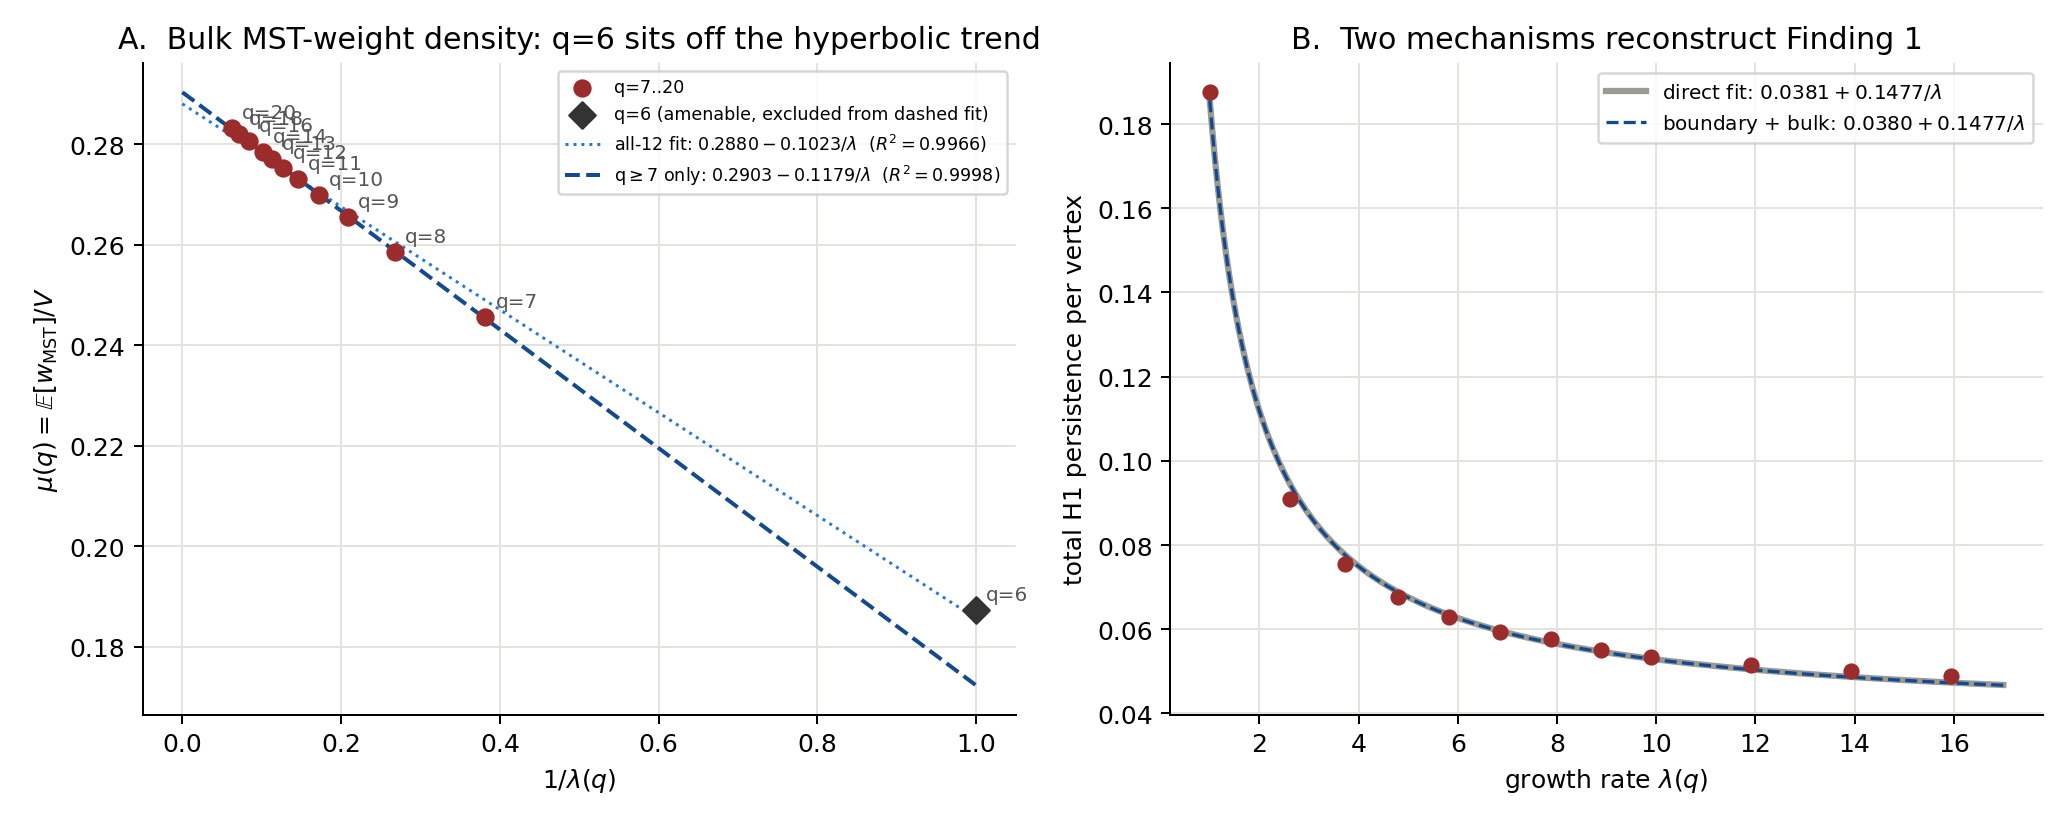
\includegraphics[width=\textwidth]{figure_mu_decomposition.png}
\caption{Left: $\mu(q)$ versus $1/\lambda(q)$, all-twelve fit (dotted) versus hyperbolic-only fit (dashed); $q=6$ shows the same leverage pattern found for $H_1$/vertex directly (\S\ref{sec:q6-outlier}). Right: the directly-fitted \S\ref{sec:scaling-law} law (grey) versus the sum of the two independently-derived mechanisms (dashed blue), indistinguishable at this scale.}
\label{fig:mu}
\end{figure}

\paragraph{$q=6$'s leverage, resolved exactly.} $\mu(q)$ shows the same pattern flagged in \S\ref{sec:q6-outlier} for $H_1$/vertex directly. Fitting only the eleven hyperbolic points gives an even tighter law, $\mu(q)=0.29031-0.11795/\lambda(q)$, $R^2=0.99977$ (versus $0.9966$ for all twelve), and extrapolating it to $\lambda=1$ predicts $\mu(6)=0.17236$, a gap of $-0.01503$ from the measured value. This is the same anomaly flagged in \S\ref{sec:q6-outlier}, not a second, independent one: since the boundary term vanishes at $q=6$, this gap and $H_1$/vertex's own gap ($-0.01551$) should be identical in the $N\to\infty$ limit, and they agree to within $0.0005$, an independent confirmation that identity \eqref{eq:reduced-identity} correctly locates $q=6$'s entire deviation from the hyperbolic trend in the bulk term, as the vanishing boundary term requires. A further cross-check comes from a completely different computational route (Kruskal MST density here, versus full persistent homology in \S\ref{sec:convergence}): the two independently measured $q=6$ asymptotes, $\mu(6)=0.18739$ and $H_1/\text{vertex}(6)=0.18757\pm0.00034$, agree to within $0.1\%$, exactly the equality this decomposition predicts.

So the scaling law of \S\ref{sec:scaling-law} is now fully accounted for, though not yet fully \emph{proven}. The boundary term is a derived consequence of the ring recursion that defines $\lambda(q)$, and the bulk term, while not yet derived from first principles, is shown to obey a comparably clean $1/\lambda(q)$ law in its own right, independently measured and sufficient to reconstruct the whole law to four significant figures. What remains open is narrower than before: the question is no longer why $H_1$ persistence scales this way, but specifically why the expected minimum-spanning-tree weight per vertex on a $\{3,q\}$ disk is itself linear in $1/\lambda(q)$. One natural route is the same recursive self-similarity that produces $\lambda(q)$: a transfer-matrix computation of $\mathbb{E}[\beta_0(p)]$ ring by ring, in the spirit of the exact solutions already available on the Bethe lattice itself. A second, more specific route: $\mathbb{E}[w_{\mathrm{MST}}]$ on the complete graph with i.i.d.\ Uniform$[0,1]$ weights is famously solvable in closed form, converging to $\zeta(3)$ \citep{frieze1985}, via an argument that replaces the finite graph with its local weak limit, the Poisson-Weighted Infinite Tree, on which the minimum spanning forest is computable recursively because the limit is a tree \citep{aldous2004}. Whether the $\{3,q\}$ percolation complex has an analogous tractable local limit as $q\to\infty$, built from triangles rather than edges, is an open question, and probably the most promising next step toward closing this gap.

$\mu(\infty)=0.28801$ should not be read as the Bethe-lattice value in the usual sense, though: even as $q\to\infty$, the $\{3,q\}$ tiling keeps being built from filled triangles, so its large-curvature limit stays a triangulated object rather than becoming the triangle-free regular tree that ``Bethe lattice'' ordinarily denotes. It is only asymptotically tree-like at long range, consistent with, and perhaps the reason for, an intercept that is small but nonzero rather than zero.

\section{Result B: embedding percolated subsets into vector space}
\label{sec:partB}

\subsection{Motivation and method}

Section~\ref{sec:partA} measures $H_1$ on the abstract percolation complex, a quantity defined without reference to any embedding at all. This section asks what happens once a cluster is mapped into a vector space, the object a downstream model (here a sparse autoencoder, or SAE) actually receives as input.

Each subcritical percolation cluster (bond percolation at $p\approx0.75$--$0.85\,p_c$, well below the critical threshold, so clusters are finite) is embedded via a \textbf{branching random walk (BRW)}: a breadth-first-search (BFS) spanning tree of the cluster is chosen, each tree edge is assigned an i.i.d.\ Gaussian step, and each node's coordinate is the cumulative sum of steps along its unique path from the cluster's root. By construction this reproduces the tree's own path metric exactly. For a non-tree (cycle-closing) edge of the cluster, though, the coordinate difference implied by the embedding generally does not equal the step that edge would have contributed, since the embedding never saw that edge at all. The \textbf{cycle inconsistency} of a cluster is the RMS norm of this holonomy, the embedded coordinate mismatch, over all of the cluster's non-tree edges: a direct, zero-assumption measurement, since no homology computation is involved, only the embedding coordinates and the already-known list of which edges are non-tree.

An SAE (ReLU encoder, unit-norm decoder columns, L1 sparsity penalty, decoder columns renormalized after each optimizer step) is then trained on the pooled BRW node embeddings for each $q$. The \textbf{feature-splitting score} for a cluster is the number of dictionary atoms needed, via greedy argmax cover, to account for $\ge90\%$ of that cluster's node memberships, averaged over clusters. Splitting is a specific, well-documented SAE pathology, where a single underlying concept gets represented by several dictionary atoms instead of one, forcing a larger dictionary to reconstruct the same information \citep{bricken2023,cunningham2023}. Here the ``concept'' being split is operationalized concretely as membership in one percolation cluster, so the score is measurable without any subjective judgment of what an atom means.

Cluster counts must be equalized across $q$ before training: at matched lattice sizes, low-$q$ lattices produce more percolation clusters than high-$q$ lattices, and without subsampling this trains a tighter SAE basis for low $q$, spuriously lowering its apparent splitting score independent of any real loop-content effect.

\subsection{Results}

Table~\ref{tab:partB} reports cycle inconsistency and feature-splitting score across four representative values of $q$, alongside the corresponding $H_1$/vertex values from Table~\ref{tab:altfit}'s underlying sweep, using $2000$ clusters per $q$ (balanced), a dictionary of $1024$ atoms, $300$ training epochs, and BRW embedding dimension $128$.

\begin{table}[htbp]
\centering
\begin{tabular}{rrrr}
\toprule
$q$ & feature-splitting score & cycle inconsistency & $H_1$/vertex \\
\midrule
7  & $4.837\pm1.393$ & 0.2775 & 0.0910 \\
8  & $4.798\pm1.348$ & 0.1940 & 0.0755 \\
12 & $4.714\pm1.274$ & 0.0986 & 0.0578 \\
20 & $4.566\pm1.180$ & 0.0297 & 0.0488 \\
\bottomrule
\end{tabular}
\caption{Feature-splitting score (mean $\pm$ SD across clusters, $n=2000$/$q$), cycle inconsistency, and $H_1$/vertex, by $q$.}
\label{tab:partB}
\end{table}

Both cycle inconsistency and feature-splitting score are monotone in $q$, in the expected direction: more loopy clusters (low $q$) require more dictionary atoms to cover the same fraction of node memberships, and produce larger embedding-space holonomy. Per-cluster splitting scores are noisy (SD $\approx1.2$--$1.4$), but at $n=2000$ clusters/$q$ the standard error of the mean is small ($\approx0.03$): the $q=7$ vs.\ $q=20$ difference is significant at $p=3.4\times10^{-11}$ (Welch $t$-test), and the pooled Spearman correlation across all $8000$ cluster-level scores is $\rho=-0.065$, $p=5\times10^{-9}$, a small effect size but a real one. The figure generated by this campaign (\texttt{campaign/figure\_feature\_splitting\_campaign.py}, \texttt{campaign/results/sae\_feature\_splitting\_campaign.png}) separates the per-cluster spread from the tighter precision of the per-$q$ mean.

The aggregate (per-$q$) feature-splitting mean also regresses against $H_1$ persistence per vertex ($r=0.93$, $p=0.07$) and against cycle inconsistency ($r=0.95$, $p=0.048$). Only 4 degrees of freedom are available here, so these $p$-values are marginal and this check is far less conclusive than \S\ref{sec:results-check}'s twelve-point comparison, but the relationship looks close to linear rather than just ordinal.

An earlier, smaller-scale run (300 clusters/$q$, BRW dimension 64, percolation parameters $p=0.150,0.120,0.085,0.047$ for $q=7,8,12,20$ respectively) measured cycle inconsistency alone and found the same monotone ordering (0.237, 0.113, 0.081, 0.045) at somewhat different absolute magnitudes than Table~\ref{tab:partB}. The direction of the effect is stable across both runs; the magnitudes are not identical, most plausibly because of the different cluster samples, sample sizes, and embedding dimension between the two campaigns. This should be reconciled, ideally by rerunning both measurements under one fixed configuration, before these numbers are reported as final.

\subsection{What this does and does not establish}

Agreement between \S\ref{sec:partA}'s combinatorial $H_1$ and this section's embedded, trained-model feature-splitting score is a real finding rather than a tautology: an embedding can create or destroy loop structure relative to the underlying complex, and a trained model's behavior is a further step removed from the embedding itself. That the two track together here means curvature's suppression of loop content survives being filtered through one specific embedding scheme (BRW, which is exact on trees by construction and about as favorable a case as an embedding can offer) and one specific downstream architecture. It does not establish that the tracking holds for other architectures, other embeddings, or the critical regime. Whether it survives embeddings that do not privilege a spanning tree (spectral embeddings, say, or a spring model with non-tree edges included as constraints), other SAE variants (TopK-SAE would remove the sparsity-level confound between architectures), or measurements taken near $p_c$ rather than well below it, is left open.

\section{Application: percolation-based data models for interpretability research}
\label{sec:brill}

Percolation-based synthetic data models for mechanistic interpretability research are one concrete setting where the tree-likeness question measured above already matters in practice. Principles of Intelligence's published data model treats a data distribution as a critical percolation cluster process on a high-dimensional lattice, generated by an explicit hierarchical fine-graining algorithm and embedded into a vector space via a branching random walk, the same embedding construction used in \S\ref{sec:partB} \citep{brill2024,brill2025lattice}. The high-dimensional case is analytically tractable because, in high dimensions, a random path essentially never self-intersects, so percolation clusters are vanishingly unlikely to contain loops; the lattice can then be replaced by a Bethe lattice, an infinite tree of fixed degree, for which the percolation threshold and critical exponents are solvable exactly \citep{brill2025lattice,stauffer1994}.

This is a homological claim dressed in probabilistic language: it says $H_1$ of the percolation cluster vanishes in the relevant limit, leaving only $H_0$ (connectivity), which is all the tree picture needs. \S\ref{sec:partA} turns ``is the treelike approximation good enough'' from a qualitative appeal to dimension into a number: total $H_1$ persistence per vertex is $0.0381+0.1477/\lambda(q)$, a finite, invertible law rather than an asymptotic statement about $d\to\infty$. Given a target loop-persistence value, the fitted law inverts directly, picking off the curvature (or, between integer $q$, an interpolated tiling family) that hits any specified distance from the treelike limit. The high-dimension argument alone cannot offer that: it only ever says the approximation gets better, not by how much at any particular finite $d$.

\S\ref{sec:partB} adds a check the original data-model literature does not: whether the same suppression, measured on the abstract complex, actually reaches a trained model's learned features once the data is embedded and used for training, rather than remaining a fact about the input distribution's own combinatorics that a downstream model might or might not pick up on. The two tracking together here is evidence, though not proof, that a data model's tree-likeness at the input level is something a trained model's own representations can inherit, not just a modeling convenience.

Two things this paper does not claim. First, it is not a demonstration that Brill's model is right or wrong in the high-dimensional regime it is actually intended for: for $d\gtrsim6$, percolation clusters have fractal dimension $4<d$, and the model's own asymptotic argument already applies on its own terms, without needing curvature as a substitute. Second, curvature and dimension are not interchangeable in general. What is shown here is that they produce the same qualitative mechanism (tree-likeness driven by an isoperimetric, non-amenability property, rather than by literal high-dimensional sparsity), not that they are numerically equivalent knobs. Curvature's real advantage is that it is a controllable, finite-size, quantifiable stand-in for a question that is otherwise only answerable in an asymptotic limit: it can be measured and dialed on graphs small enough to simulate directly, which the high-dimensional case is not.

% Sections 7 (Discussion and open questions) and 8 (pipeline/code appendix) per
% PAPER_OUTLINE.md are not yet drafted.

\bibliographystyle{plainnat}
\bibliography{references}

\end{document}
